%\documentclass{beamer}
\documentclass[RawSienna,dvipsnames]{beamer}

%%% Dichiarazione dei pacchetti standard.
\usepackage[italian]{babel}
\usepackage[utf8x]{inputenc}
%%% Personalizzazione del layout---articolata su cinque livelli.
%\usetheme{split}        % layout complessivo. 
\usetheme{CambridgeUS}
\useinnertheme{rectangles} % layout interno.
\useoutertheme{infolines} % layout esterno.
\setbeamercolor{title}{fg=RawSienna}
\setbeamercolor{frametitle}{fg=RawSienna}
\usecolortheme{crane} % schema di colori.
\usefonttheme{professionalfonts}  % schema dei font.
\setbeamercolor{item}{fg=RawSienna}
% Inutile dire che se volete tutti i default, potete risparmiarvi gli ultimi
% quattro comandi. 

%%% Titolo e autore.
\title{Monolith}
\subtitle{An interactive bubble provider}
\author{Revisione di Progettazione}
%\institute{Gruppo Utilizzatoti Italiani di \TeX}
%\date{\today}
\date{27 giugno 2017}

\begin{document}

\section{Scopo del progetto}
\begin{frame}
	\frametitle{Scopo del progetto}
	\begin{center}
	\begin{large}
		\textbf{Monolith}: Framework per la creazione di bolle interattive \\
		\vspace{1cm}
		\textbf{Demo}: Bolla esempio che usa Monolith
	\end{large}
	\end{center}
	
\end{frame}

\section{Copertura dei Requisiti}
\begin{frame}
	\frametitle{Copertura dei Requisiti}
	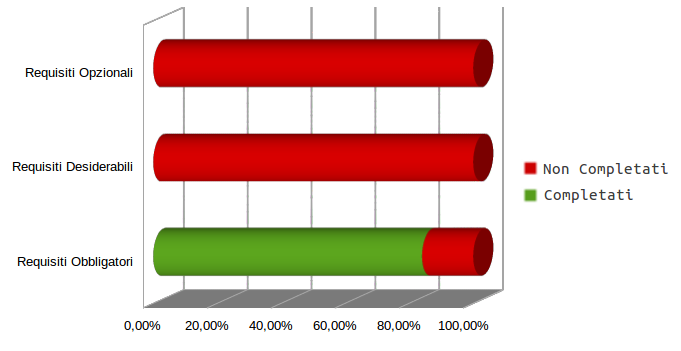
\includegraphics[scale=0.50]{img/Requisiti.png}
	
\end{frame}

\section{Lavori da ultimare}
\begin{frame}
	\frametitle{Lavori da ultimare}
	
	\begin{columns}
		\begin{column}{0.4\textwidth}
			
		\end{column}
		
		\begin{column}{0.5\textwidth}
			\begin{itemize}
				\begin{Large}
				\item Codice
				\vspace{0.5cm}
				\item Manuali
				\vspace{0.5cm}
				\item Test
				\end{Large}		
			\end{itemize}
		\end{column}
		
		\begin{column}{0.2\textwidth}
			
		\end{column}
	\end{columns}
	
\end{frame}

\section{Test}

\subsection{Stato dei Test}
\begin{frame}
	\frametitle{Stato dei Test}
	\begin{center}
	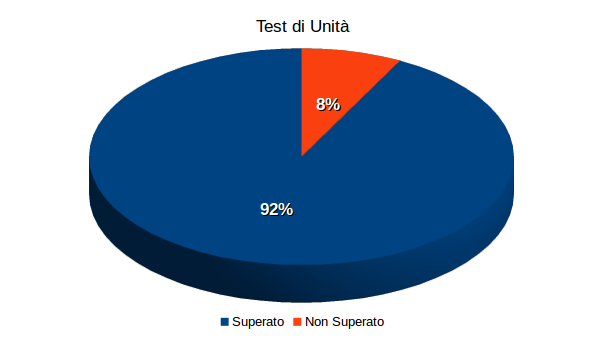
\includegraphics[scale=0.55]{img/TU.png}
	\end{center}
\end{frame}

\begin{frame}
	\frametitle{Stato dei Test}
	\begin{center}
	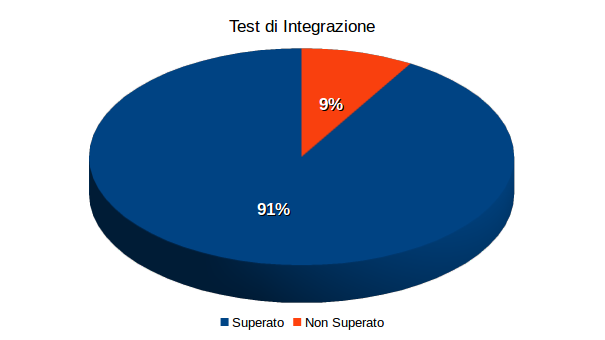
\includegraphics[scale=0.55]{img/TI.png}
    \end{center}
\end{frame}

\begin{frame}
	\frametitle{Stato dei Test}
	\begin{center}
	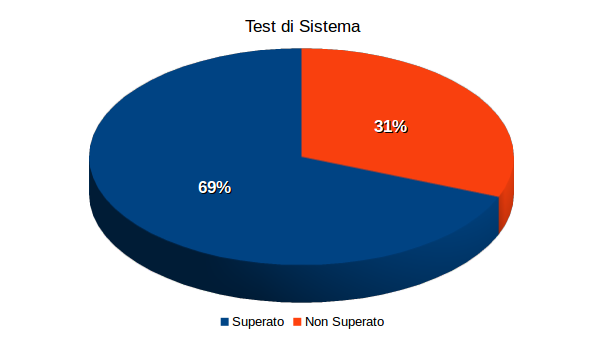
\includegraphics[scale=0.55]{img/TS.png}
    \end{center}
\end{frame}

\subsection{Strumenti usati}
\begin{frame}
	\frametitle{Strumenti usati}
	\begin{center}
	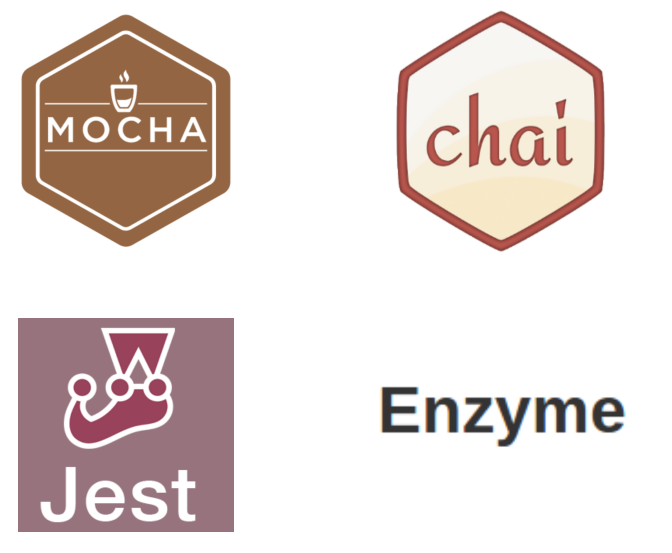
\includegraphics[scale=0.30]{img/strumenti.png}
	\end{center}
\end{frame}
 %fede


\section{Descrizione Architettura SDK}
\subsection{Visione ad alto livello}
\begin{frame}
  \frametitle{Diagramma dei package}
  \begin{center}
    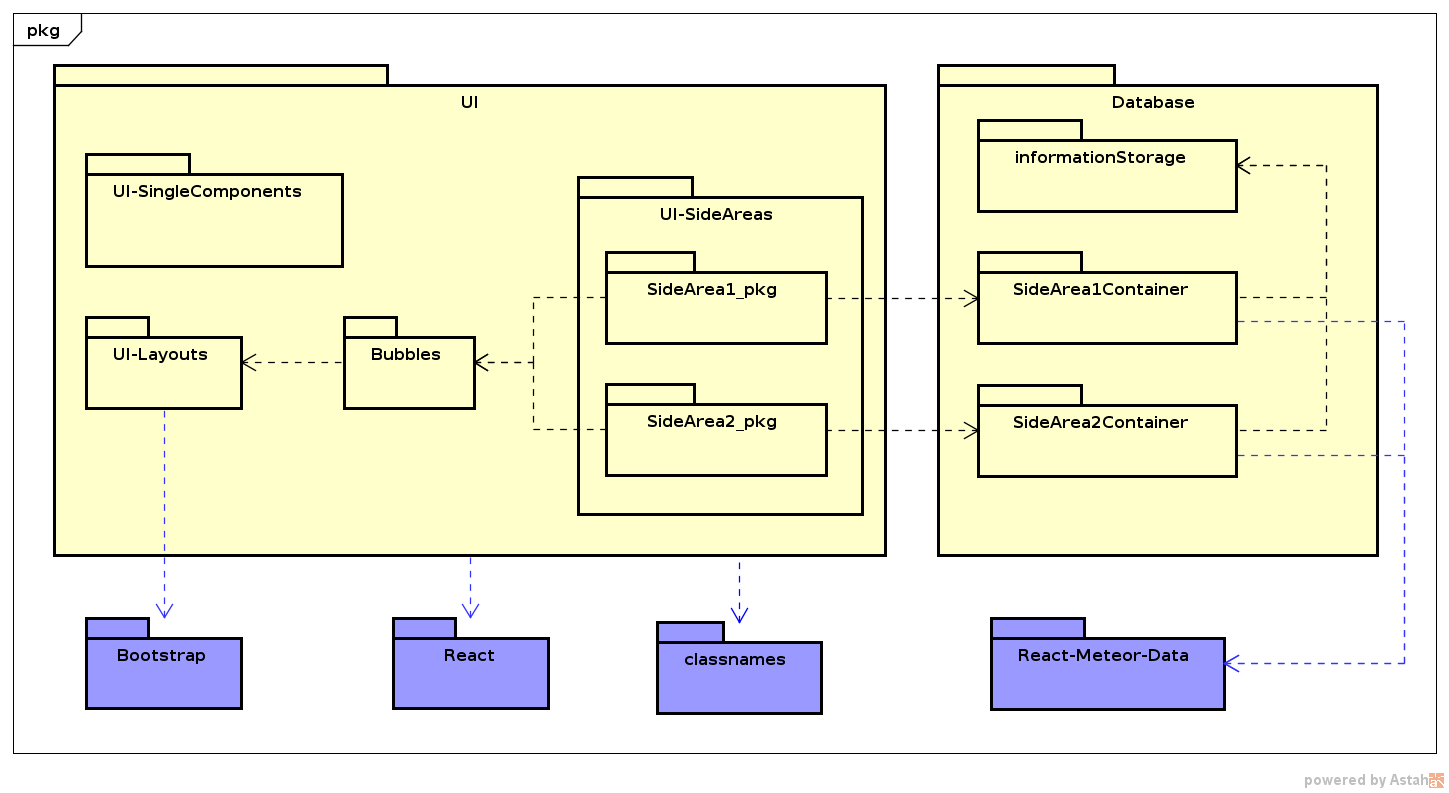
\includegraphics[scale=0.30]{img/General.png}
  \end{center}
\end{frame}


\begin{frame}
  \frametitle{Flusso dei dati }
  \begin{center}
    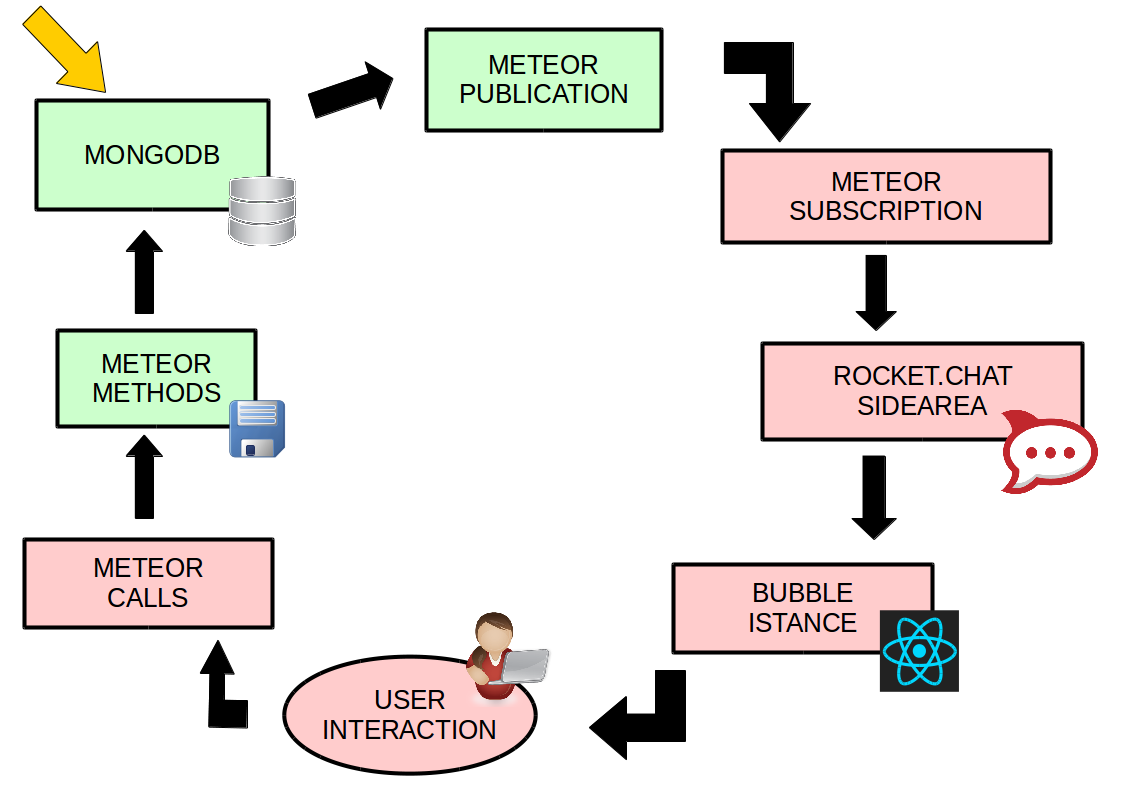
\includegraphics[scale=0.30]{img/2flussodati.png}
  \end{center}
\end{frame}


\subsection{Visione di dettaglio}

\begin{frame}
  \frametitle{Configurazione Database }
  \begin{center}
    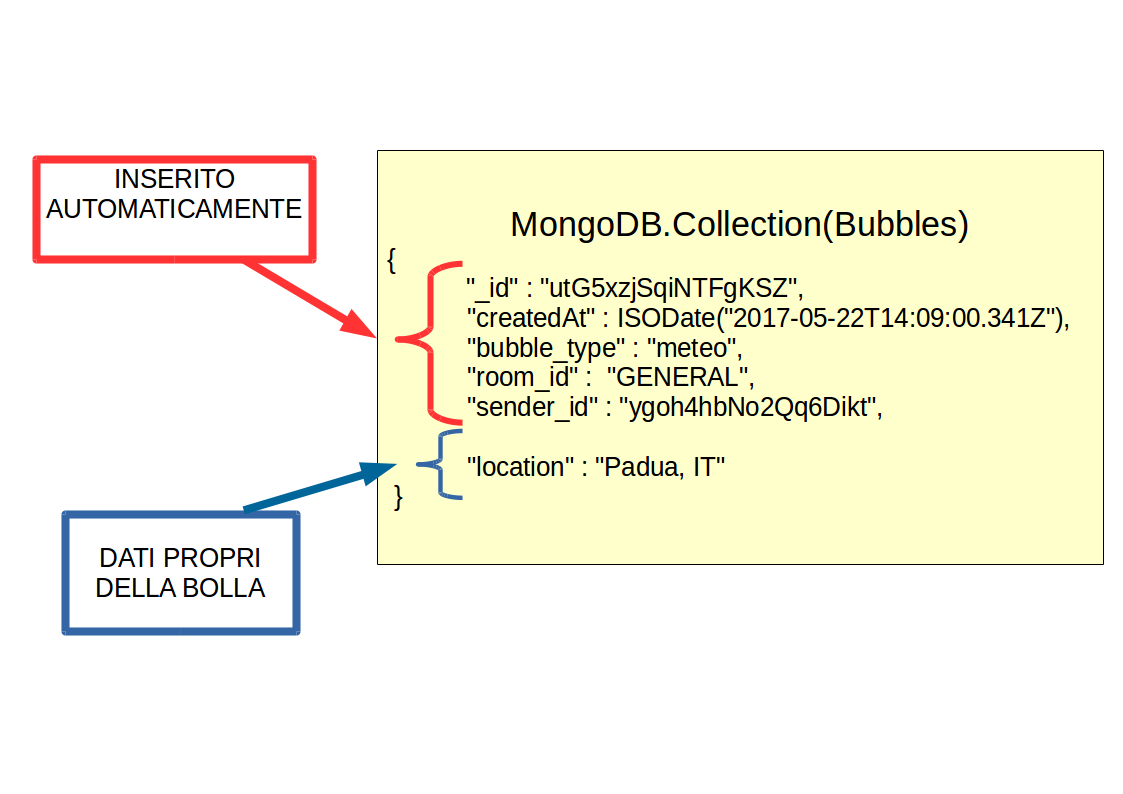
\includegraphics[scale=0.28]{img/1mongo.png}
  \end{center}
\end{frame}


\begin{frame}
  \frametitle{Pubblication \& subscription }
  \begin{center}
    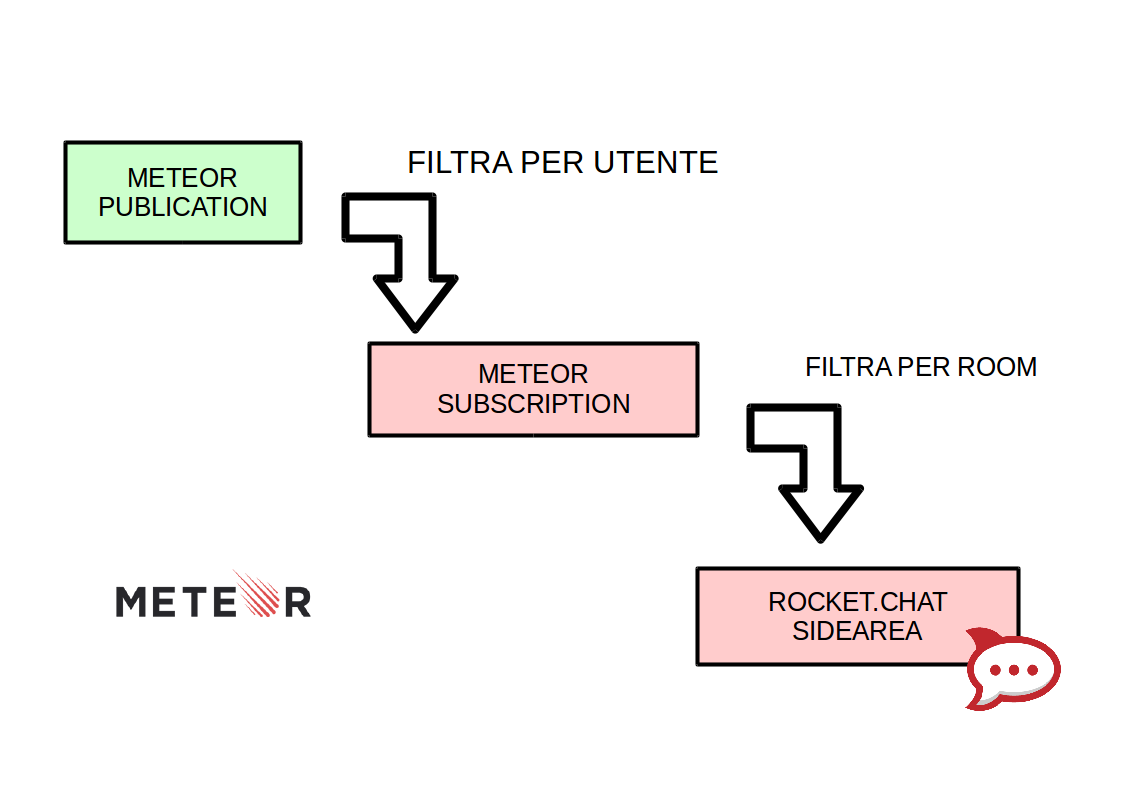
\includegraphics[scale=0.28]{img/3publication.png}
  \end{center}
\end{frame}


\begin{frame}
  \frametitle{Creazione delle bolle }
  \begin{center}
    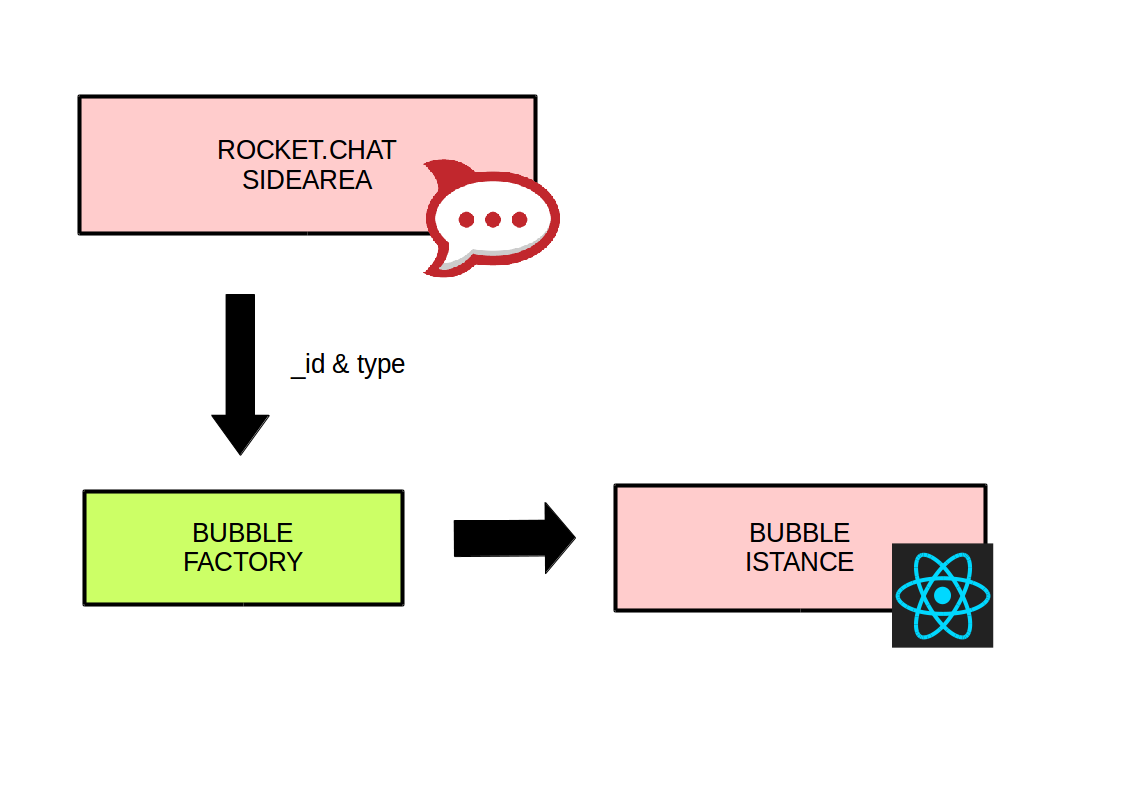
\includegraphics[scale=0.28]{img/4bubbles.png}
  \end{center}
\end{frame}

\begin{frame}
  \frametitle{Diagramma classi per le componenti grafiche }
  \begin{center}
    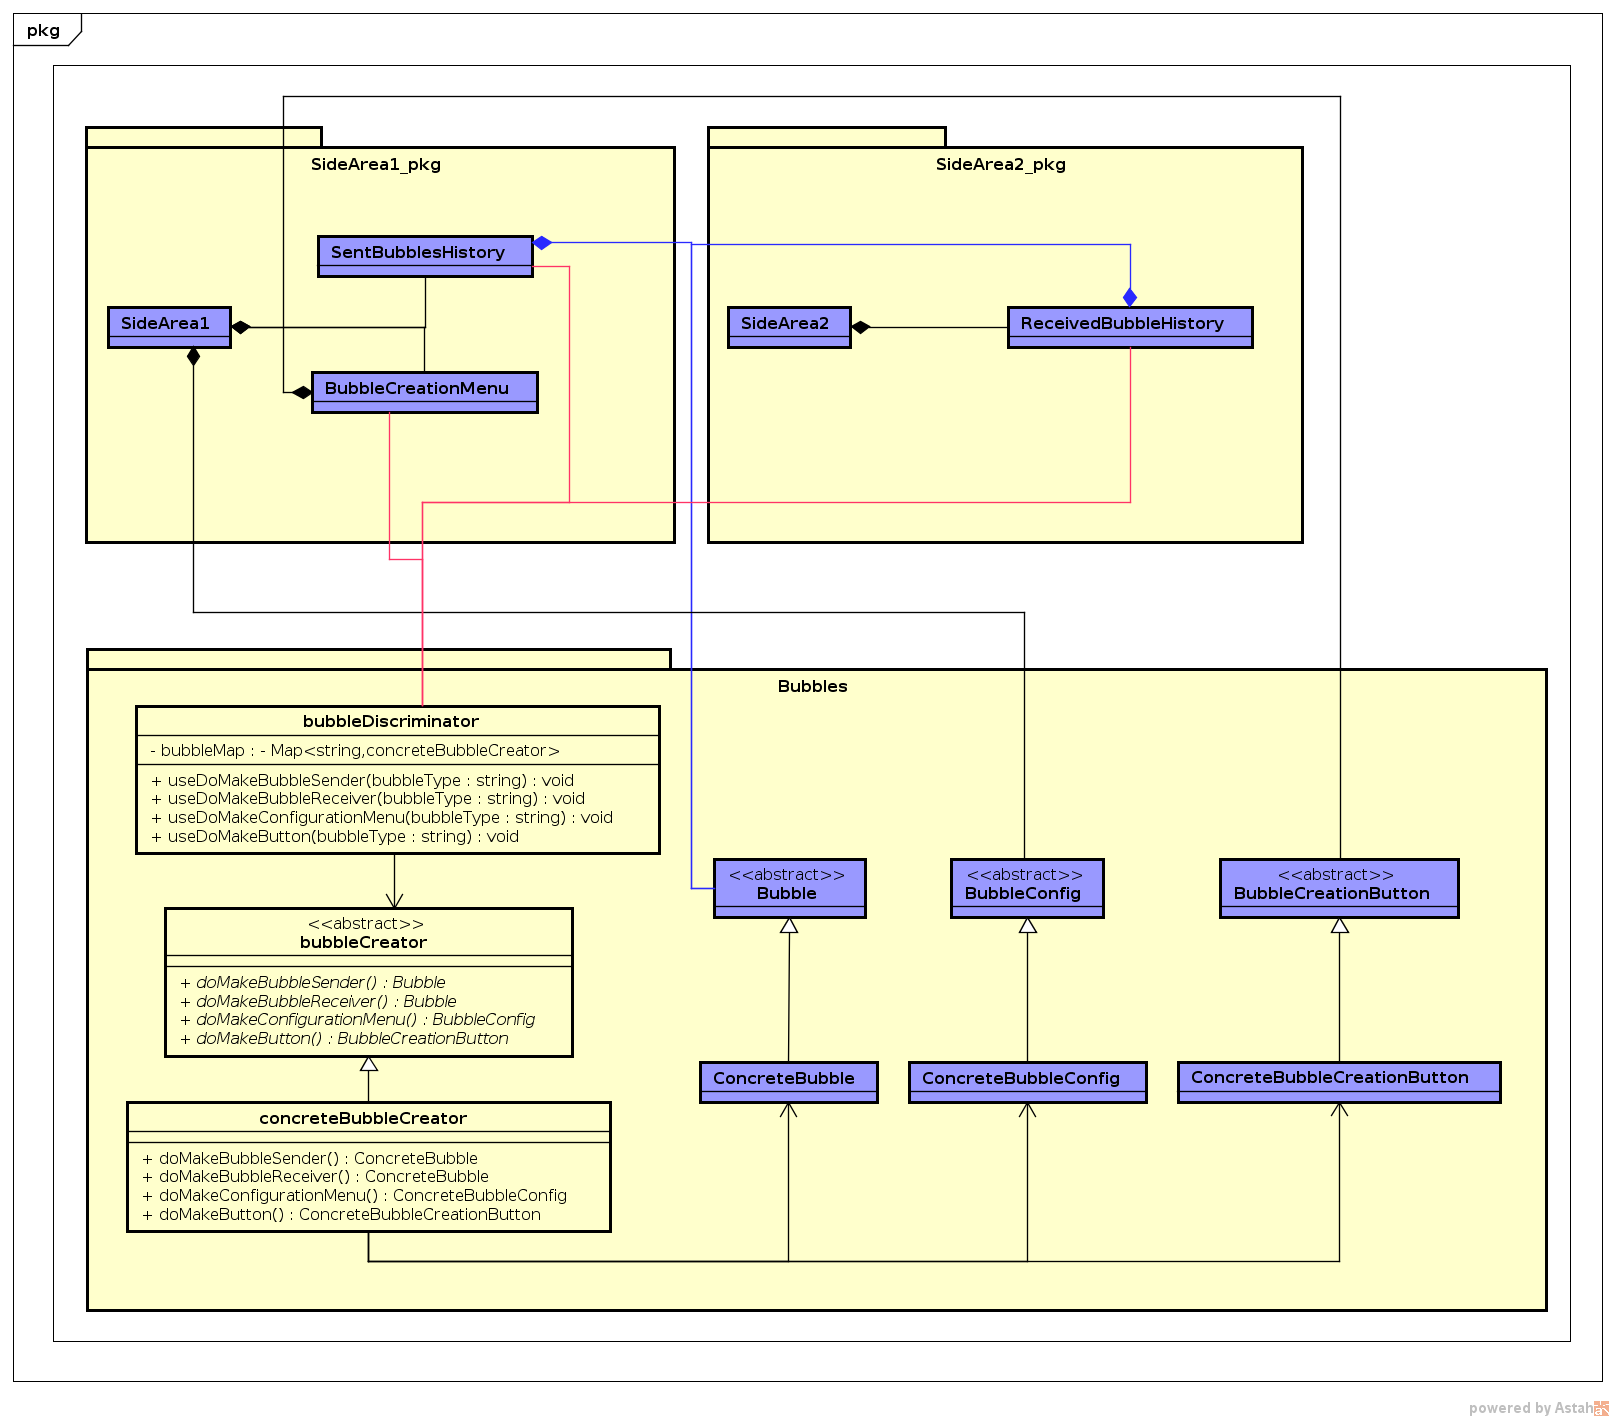
\includegraphics[scale=0.20]{img/Bubbles.png}
  \end{center}
\end{frame}


\begin{frame}
  \frametitle{Meteor.call \& Meteor.methods }
  \begin{center}
    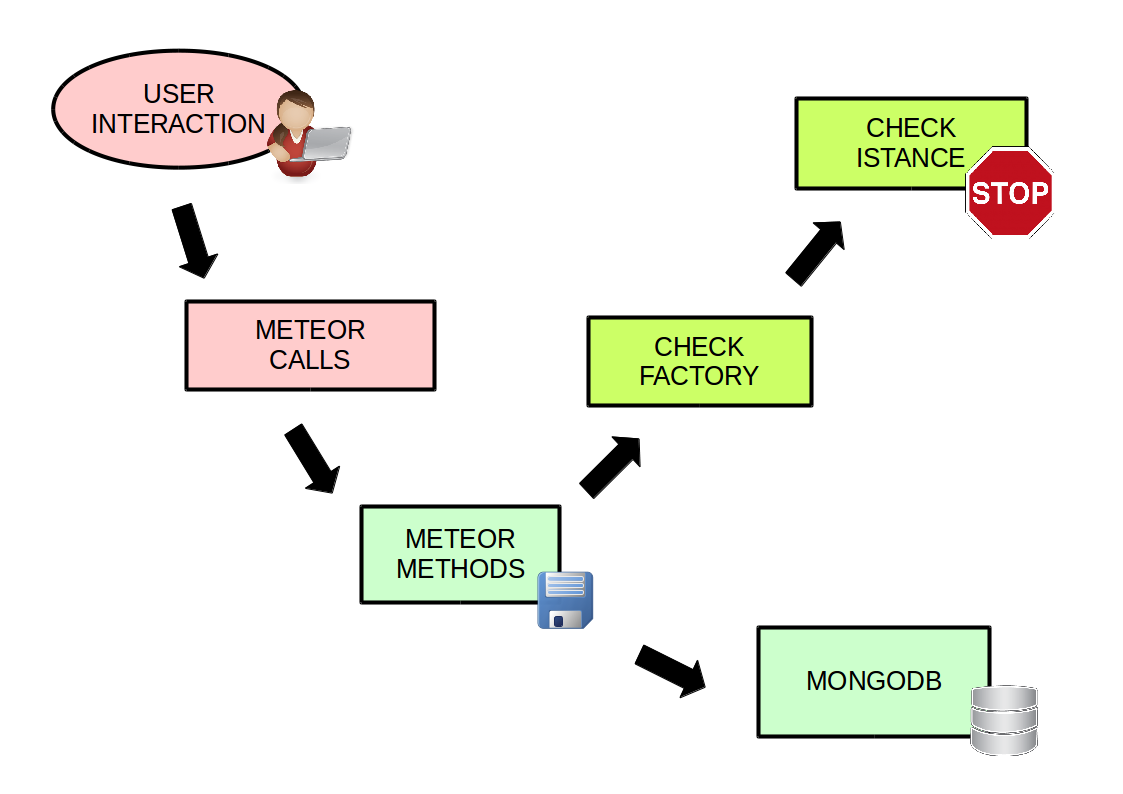
\includegraphics[scale=0.28]{img/5methods.png}
  \end{center}
\end{frame}
 %nicolò e tomas

\section{Descrizione prodotto}




\begin{frame}
	\frametitle{Funzionamento SDK}
\begin{center}
	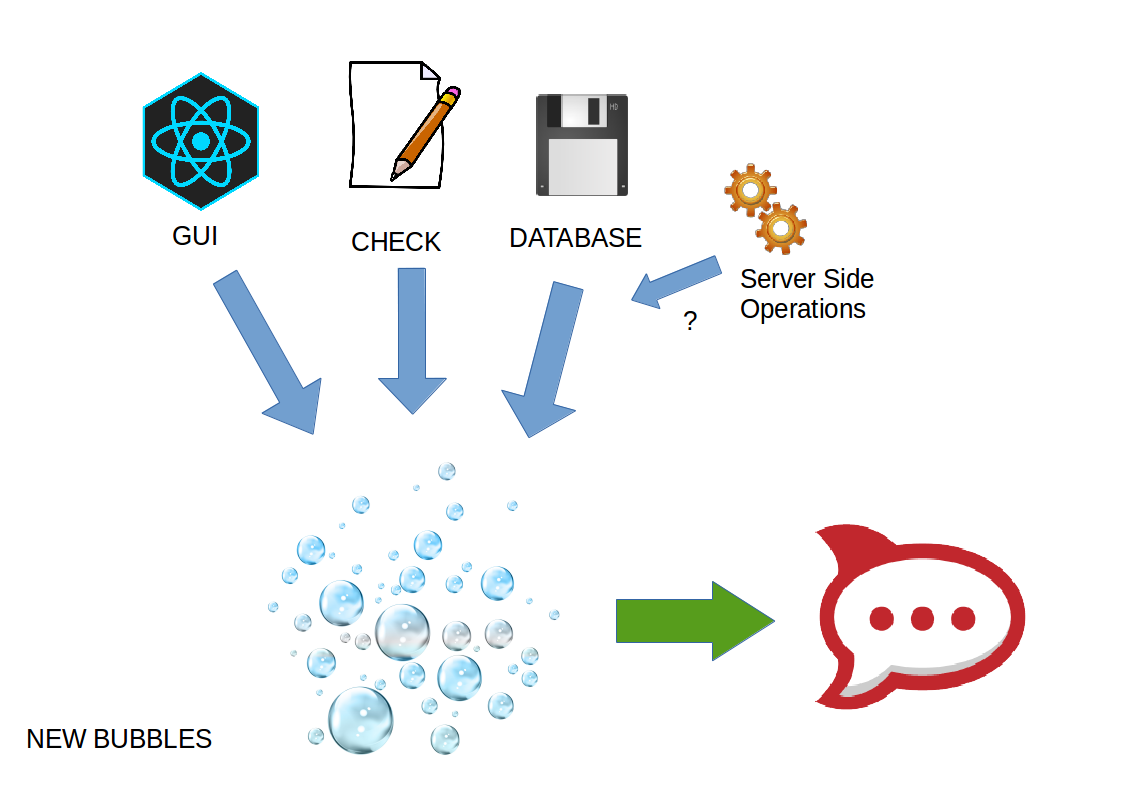
\includegraphics[width=\linewidth,height=.8\textheight,keepaspectratio]{img/uso_sdk.png}
\end{center}
\end{frame}
 %emanuele

\section{Modifiche Apportate}
\subsection{Generali}

\begin{frame}
	\frametitle{Modifiche Generali}
	
		
		\begin{columns}
			\begin{column}{0.2\textwidth}
				
			\end{column}
			
			\begin{column}{0.4\textwidth}
				\begin{itemize}
					\item Numero di versione per documento
					\item Registro delle modifiche
					\item Verbali
				
				\end{itemize}
			\end{column}
			
			\begin{column}{0.2\textwidth}
				
			\end{column}
		\end{columns}
		
		
\end{frame}


\subsection{Documenti}

\begin{frame}
	\frametitle{Modifiche Documenti}
	
	
	\begin{columns}
		\begin{column}{0.2\textwidth}
			
		\end{column}
		
		\begin{column}{0.4\textwidth}
			\begin{itemize}
				\item Norme di Progetto
				\item Analisi dei Requisiti
				\item Piano di Progetto
				\item Piano di Qualifica
				
			\end{itemize}
		\end{column}
		
		\begin{column}{0.2\textwidth}
			
		\end{column}
	\end{columns}
	
\end{frame} %silvio

\section{Preventivo e Consultivo}
%\subsection{Progettazione Architetturale}
\begin{frame}
  \frametitle{Progettazione Architetturale}
  \begin{center}
  	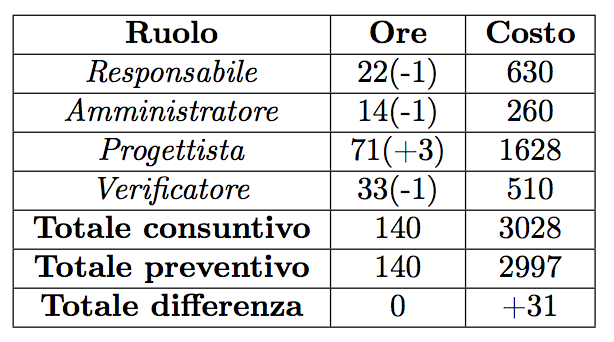
\includegraphics[scale=0.5]{img/prevPA}
  	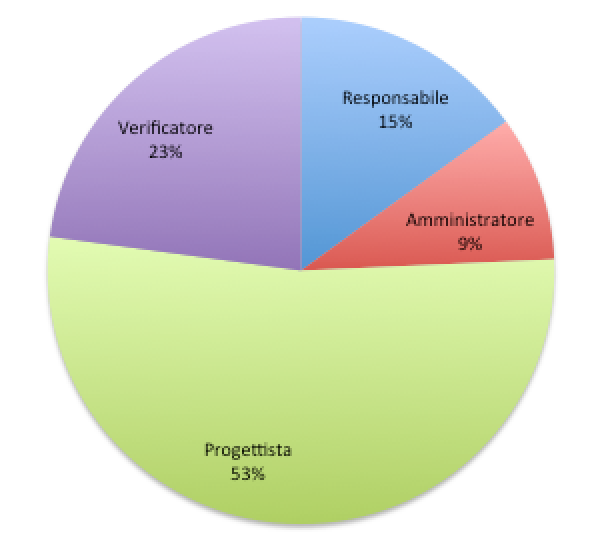
\includegraphics[scale=0.4]{img/cakePA}
  \end{center}
Rispetto al preventivo, sono emerse differenze con una diminuzione di 1 ora sui ruoli di Responsabile, Amministratore e Verificatore, ed una maggiorazione di 3 ore per quello del Progettista.
\end{frame}

\begin{frame}
	\frametitle{Progettazione di Dettaglio}
	\begin{center}
		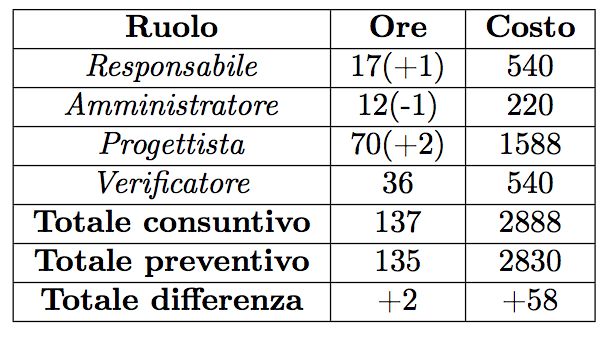
\includegraphics[scale=0.5]{img/prevPD}
		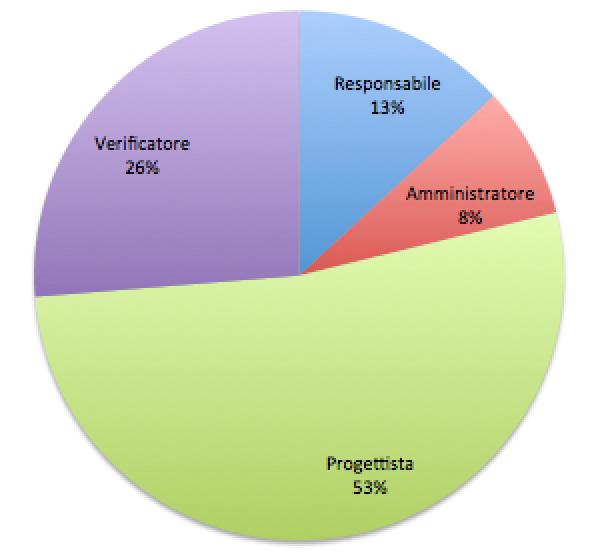
\includegraphics[scale=0.4]{img/cakePD}
	\end{center}
	Rispetto al preventivo, sono emerse differenze con una diminuzione di 1 ora sul ruolo di Amministratore  ed una maggiorazione sui ruoli di  Amministratore e Progettista.
	
\end{frame} %riccardo

\end{document}
